\section{Laboratory work implementation}

\subsection{Analiza lucrării de laborator}

	https://github.com/MarinaJechiuTI154/MIDPS - linkul repozitoriului.

	Principalele noțiuni cu care voi opera:
	\begin{itemize}
	\item \textbf{repository}  componenta server ce conține informații privind ierarhia de fișiere și reviziile.
	\item \textbf{branch} este o ramură secundară de dezvoltare a unui proiect.
	\item \textbf{checkout}  preluarea în mediul local a unei anumite revizii publicate pe server.
	\item \textbf{commit} cerere de publicare pe server a unor modificări.
	\item \textbf{pull} acțiunea de actualizare (update) a informațiilor locale cu cele de pe server.
	\item \textbf{conflict} apare atunci când mai mulți utilizatori vor să publice modificări aplicate acelorași fișiere din proiect, însă sistemul de aplicare a versiunilor diferite nu poate îmbina modificările.
	\item \textbf{revert} revenirea la o versiune anterioară pe un anume fir de dezvoltare (branch).
	\item \textbf{tag} branch “read-only” ce nu mai permite modificări ulterioare (folosit uneori pentru versiunile stabile și derivă dintr-un branch)
	\end{itemize}
	
	Am creat un cont public pe github cu denumirea mdps. Pentru a putea gestiona repozitoriul am instalat GitBash. Pentru a activa contul avem nevoie sș introducem în  setări cheia, care se obține prin tastarea în linia de comandă: ssh-keygen. Pentru a deschide cheia obținută folosim următoarele instrucțiuni:  cat ~ /.ssh /id - rsa.pub. Pentru a face legătura între repozitoriul pe github și cel local este necesar să clonăm repozitoriul online cu instrucțiune: \textit{git clone}.
	
	La crearea repozitoriului se creează un branch implicit numit master. Însă, dacă trebuie să creăm un nou branch folosim comanda:\textit{git checkout 'denumire-branch'}. Astfel, nu doar se creează un nou branch, dar și se trece automat pe acest branch. În cazul în care dorim să trecem pe un branch deja existend, la tastarea denumirii acestuia sistemul îl recunoaște și face automat salt către acesta. 
	
	Deoarece repozitoriile git sunt repozitorii de tip distrib, pentru a încărca modificările efectuate local pe server este necesar penrtu a efectua următoarii pași: \begin{list}{•}{}
	\item  \textit{git add .} adăugarea în index a modificărilor realizate în directoriul meu, fișiere ce se intenționează a fi publicate.
	\item  \textit{git commit} efectuarea commit-urilor în baza informației din index. Acestea pot conține denumiri pentru a gestiona mai ușor modificările.
	\item \textit{git push} publicarea modificărilor pe repozitoriu.
	\end{list}
	
	Pentru a putea face push pe branch-urile create, este necesar ca acestea să fie setate to track a remote origin. Pentru asta vom folosi comanda: \textit{git push -u origin den-branch}. 
	
	Ultimul commit efectuat în repozitoriu poartă numele de HEAD. Astfel, pentru a reveni la un commit anterior este suficient să scriem în linia de comandă: \textit{git reset --hard HEAD}.
	
	Uneori, vrem să facem anumite schimbări temporare, dar fără a face deodat[ commit asupra acestora. Pentru asta utilizăm comanda \textit{git stash}. Putem totodată să revenim asupra acestor modificări mai tîrziu.
	
	Nu întotdeauna dorim sa versionăm anumite fisiere, întrucât acestea pot conține executabile generate de procesul de compilare sau efectiv parametrii de configurare ai aplicației. Fișierele sau directoarele ce se doresc a fi ignorate de sistemul de versionare pot fi trecute într-un fișier numit .gitignore. Acesta este evaluat in mod recursiv, putand astfel avea mai multe fișiere .gitignore în folderele proiectului nostru. Cu toate acestea, pentru a nu căuta foarte mult path-urile ignorate, se folosește în mod convențional un singur astfel de fisier plasat în radacina proiectului. În momentul în care încărcăm un fișier ce are o extensie menționată în fișierul .gitignore, acesta este pur și simplu ignorat și nu este încărcat pe repozitoriu.
	
	După crearea a două sau mai multe branch-uri acestea sunt dezvoltate separat, conținând informații diferite deobicei. Dacă dorim să unim aceste două branch-uri într-unul singut folosim comanda \textit{git merge}. Aceasta se va executa numai dacă între aceste branch-uri nu există conflict, adică conținutul lor este identic. Pentru a rezolva aceste conflicte trebuie sincronizate cele două branch-uri, ambele să aibă informație identică.
	
	În istoria modificărilor pot fi marcate cele mai importante modificări cu ajutorul tag-urilor. Git-ul folosește două tipuri de tag-uri: simple și adnotate. Numele tag-urilor au următoarea formă: v0.1, v3.4 etc. Pentru a inițializa un gat adnotat introducem: \textit{git tag -a v1.2 -m ”nume-tag”}. Tag-urile adnotate sunt stocate ca obiecte complete în baza de date. Tag-ul ușor este de fapt un pointer către un anumit commit. Acesta se inițializează: textit{git tag v1.2 -lw}.
	
	
\subsection{Imagini}
\begin{figure}[h]
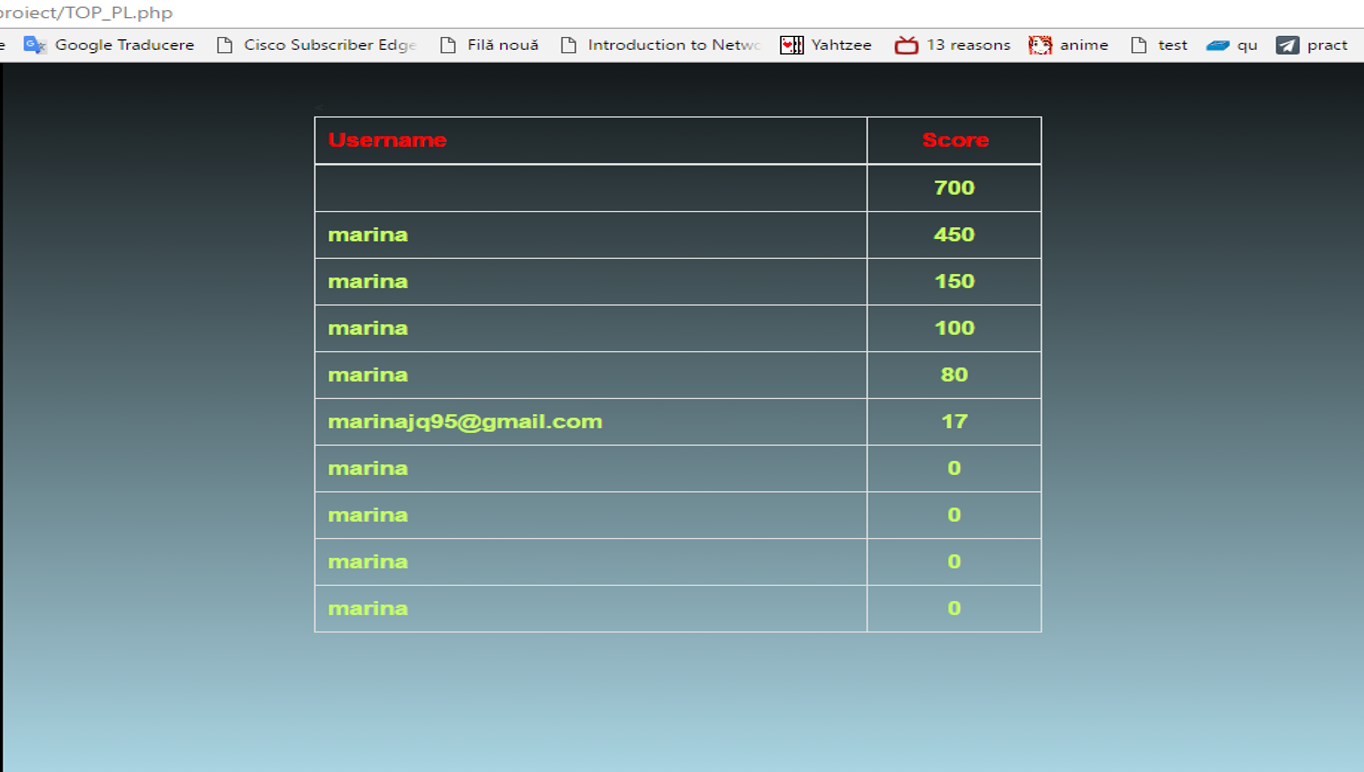
\includegraphics[width=0.8\textwidth]{1}
\caption{Trecerea de pe un branch pe altul}
\label{fig:1}
\end{figure}

\begin{figure}[h]

\includegraphics[width=0.8\textwidth]{2}
\caption{Adăugarea modificărilor efectuate din directoriu în index}
\label{fig:2}
\end{figure}

\begin{figure}[h]
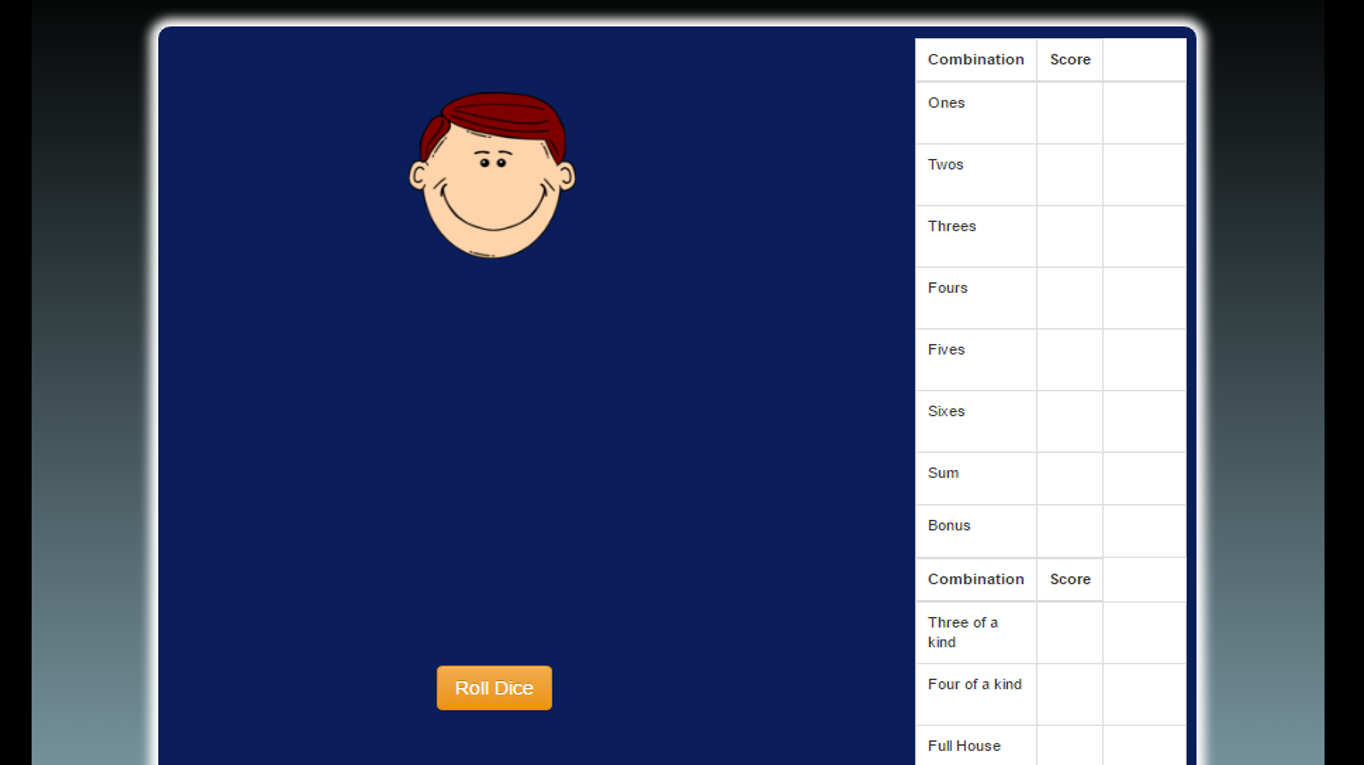
\includegraphics[width=0.8\textwidth]{3}
\caption{Comanda commit}
\label{fig:3}
\end{figure}

\begin{figure}[h]

\includegraphics[width=0.8\textwidth]{5}
\caption{Revenirea la ultimul commit}
\label{fig:4}
\end{figure}

\begin{figure}[h]
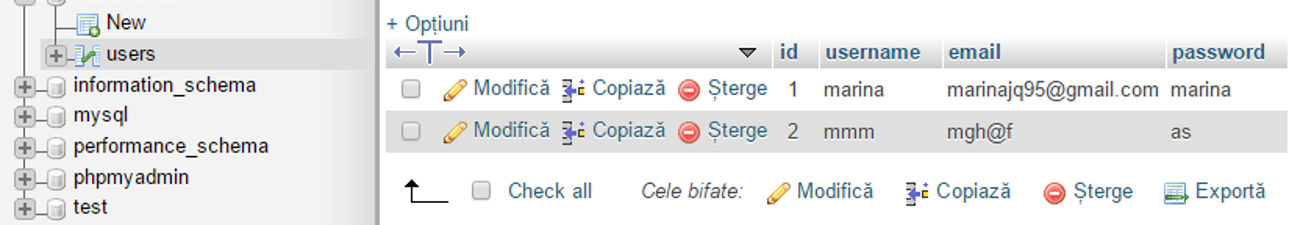
\includegraphics[width=0.8\textwidth]{7}
\caption{Salvarea temporară a modificărilor}
\label{fig:5}
\end{figure}

\begin{figure}[h]
\includegraphics[width=0.8\textwidth]{8}
\caption{Conflict}
\label{fig:6}
\end{figure}

\begin{figure}[h]
\includegraphics[width=0.8\textwidth]{9}
\caption{Imaginea grafică a repozitoriului}
\label{fig:7}
\end{figure}

\begin{figure}[h]
\includegraphics[width=0.8\textwidth]{10}
\caption{Crearea unui nou branch}
\label{fig:8}
\end{figure}

\begin{figure}[h]
\includegraphics[width=0.8\textwidth]{11}
\caption{Set a branch to track a remote origin}
\label{fig:9}
\end{figure}

\begin{figure}[h]
\includegraphics[width=0.8\textwidth]{12}
\caption{Clonarea unui repozitoriu}
\label{fig:10}
\end{figure}

\begin{figure}[h]
\includegraphics[width=0.8\textwidth]{13}
\caption{Implementarea tag-urilor}
\label{fig:11}
\end{figure}

\begin{figure}[h]
\includegraphics[width=0.8\textwidth]{14}
\caption{Ignorarea fișierului cu extensia .pfx, conform fișierului .gitignore}
\label{fig:12}
\end{figure}

\begin{figure}[h]
\includegraphics[width=0.8\textwidth]{15}
\caption{Fișiere ce le conține repozitoriul. Deși în lista apare fișierul ign.pfx, el nu este vizibil pe repozitoriu}
\label{fig:13}
\end{figure}

\clearpage